

\title{Schlüsselexperimente in der Teilchenphysik}
\author{
        Jean-Marco Alameddine \\
}
\date{\today}

\documentclass[12pt]{article}

% deutsche Spracheinstellungen
\usepackage{polyglossia}
\setmainlanguage{german}

\usepackage{suffix}

\usepackage{geometry}
\geometry{a4paper,left=25mm,right=25mm, top=3cm, bottom=3cm}

% unverzichtbare Mathe-Befehle
\usepackage{amsmath}
% viele Mathe-Symbole
\usepackage{amssymb}
% Erweiterungen für amsmath
\usepackage{mathtools}

% Fonteinstellungen
\usepackage{fontspec}
% Latin Modern Fonts werden automatisch geladen

\usepackage[
  math-style=ISO,    % ┐
  bold-style=ISO,    % │
  sans-style=italic, % │ ISO-Standard folgen
  nabla=upright,     % │
  partial=upright,   % ┘
  warnings-off={           % ┐
    mathtools-colon,       % │ unnötige Warnungen ausschalten
    mathtools-overbracket, % │
  },                       % ┘
]{unicode-math}

% traditionelle Fonts für Mathematik
\setmathfont{Latin Modern Math}
\setmathfont{XITS Math}[range={scr, bfscr}]
\setmathfont{XITS Math}[range={cal, bfcal}, StylisticSet=1]

% Zahlen und Einheiten
\usepackage[
  locale=DE,                 % deutsche Einstellungen
  separate-uncertainty=true, % immer Fehler mit \pm
  per-mode=reciprocal,       % ^-1 für inverse Einheiten
  % alternativ:
  % per-mode=reciprocal, % m s^{-1}
  % decimal-marker=., % . statt , f�r Dezimalzahlen
]{siunitx}

% chemische Formeln
\usepackage[
  version=4,
  math-greek=default, % ┐ mit unicode-math zusammenarbeiten
  text-greek=default, % ┘
]{mhchem}

% Grafiken können eingebunden werden
\usepackage{graphicx}
% größere Variation von Dateinamen möglich (Probleme mit Leerzeichen behoben)
\usepackage{grffile}

\usepackage{float}

\newcommand\chapterauthor[1]{\authortoc{#1}\printchapterauthor{#1}}
\WithSuffix\newcommand\chapterauthor*[1]{\printchapterauthor{#1}}

\makeatletter
\newcommand{\printchapterauthor}[1]{%
  {\parindent0pt\vspace*{-25pt}%
  \linespread{1.5}\large\scshape#1%
  \par\nobreak\vspace*{35pt}}
  \@afterheading%
}
\newcommand{\authortoc}[1]{%
  \addtocontents{toc}{\vskip-5pt}%
  \addtocontents{toc}{%
    \protect\contentsline{chapter}%
    {\hskip1.3em\mdseries\scshape\protect\scriptsize#1}{}{}}
  \addtocontents{toc}{\vskip5pt}%
}
\makeatother

\usepackage{xfrac}
\usepackage{url}

\begin{document}

\maketitle
\newpage

%\begin{abstract}
%This is the paper's abstract \ldots
%\end{abstract}

\setcounter{tocdepth}{1} %nicht alle Unter-Unterkapitel anzeigen (1 -> Nur Überschriften, 2-> Auch 1. Unterkapitel)

\tableofcontents
\newpage

\section{Cherenkov-Detektoren}

\chapterauthor{Rune Dominik, 26.10.2018}

\subsection{Geschichte}
Tatsächlich hat bereits Marie Curie blaues Licht gesehen, was heute als Cherenkovlicht erklärt werden kann.

\subsection{Theorie}
Der Cherenkoveffekt tritt auf, wenn geladene Teilchen mit Überlichtgeschwindigkeit durch ein Medium propagieren. Es wird hierdurch ein Cherekovlichtkegel abgegeben, siehe Abbildung \ref{fig:aufbau}.

\begin{figure}[H]
  \centering
  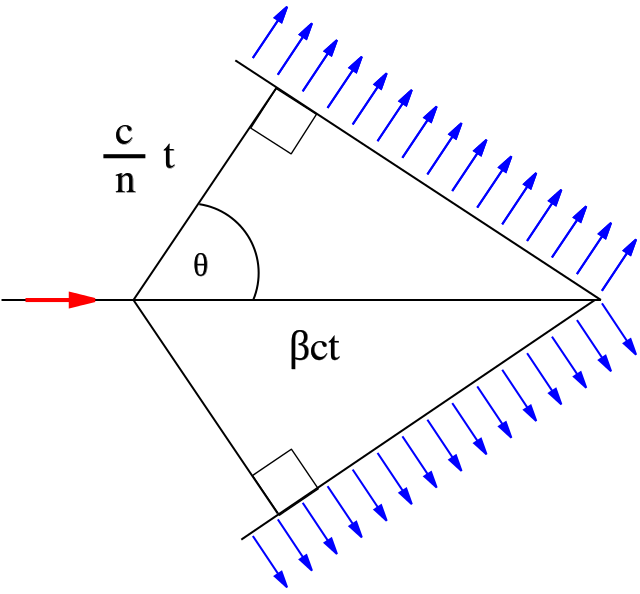
\includegraphics[height=6.0cm]{content/Cherenkov.png}
  \caption{Theoretische Erklärung des Cherenkoveffektes.}
  \label{fig:aufbau}
\end{figure}

\subsection{Aufbau}
Es gibt verschiedene Bauweisen für solche Teleskope. Insbesondere die HESE ist eine sehr moderne Bauweise.

Test~\cite{Gil:02}



\newpage


\section{Wu-Experiment}

\chapterauthor{Inga Höfmann, 02.11.2018}

\subsection{Historische Entwicklung}
Das Wu-Experiment beschäftigt sich mit der Parität, welche als Operator eine Inversion in allen Raumkoordinaten beschreibt. Es gilt
\begin{align*}
	\hat{P} \vec{r} &= -\vec{r}, &
	\hat{P} \vec{L} &= \vec{L}.
\end{align*}
Die Parität wurde erstmals im Jahre 1927 als Quantenzahl und somit intrinsische Eigenschaft eines Teilchen eingeführt und galt zunächst für alle Wechselwirkungen als erhalten.
Zweifel an der Parität als Erhaltungsgröße kamen im Jahr 1954 mit dem sogenanten $\tau$-$\theta$-Puzzle auf:
Die damals als $\tau$- und $\theta$-Meson bekannten Teilchen besaßen identische Massen, Ladungen und Lebensdauern.
Unteschiede ergaben sich lediglich in den Zerfallsprodukten:
Während das $\tau^+$-Meson in den Endzustand $\pi^+ \pi^+ \pi^-$ (Parität $-1$) zerfiel, war der Endzustand des $\theta^+$-Mesons $\pi^+ \pi^0$ (Parität $+1$).
Als Erklärung dieses Puzzles existierte die Möglichkeit, dass es sich bei beiden Mesonen um das gleiche Teilchen handelt und die Parität in diesem Fall verletzt ist.
Diese Vermutung wurde, zusammen mit Vorschlägen für einen experimentellen Aufbau, im Jahre 1957 von Tsung-Dao Lee und Chen Ning Yang in einem Paper veröffentlicht, wofür sie 1957 den Nobelpreis erhielten.
Das dazugehörige Experiment wurde von der Physikerin Chien-Shiung Wu im Jahre 1956 innerhalb von neun Monaten realisiert.

\subsection{Idee des Wu-Experimentes}
Die Idee des Wu-Experimentes ist es, eine Paritätsverletzung in der schwachen Wechselwirkungs nachzuweisen.
Um einen Interferenzterm mit paritätserhaltenden und paritätsverletzenden Anteilen untersuchen zu können muss eine pseudoskalare Messgröße genutzt werden.
Hierzu bietet es sich an, die Winkelverteilung $I\left(\theta \right)$ von $e^-$ in einem $\beta$-Zerfall zu betrachten. 
Es ergibt sich ein Parameter $\alpha$, welcher die Asymmetrie in der Winkelverteilung beschreibt, wobei $\alpha = 0$ für Paritätserhaltung bzw. $\alpha \neq 0$ für Paritätsverletzung gilt.

Das Wu-Experiment ist so konzipiert, dass es rein qualitative Aussagen über den Parameter $\alpha$ treffen kann.
Als Probe wird $\ce{^{60}_{27}Co}$ verwendet, welches dominant unter Aussendung eines $e^-$ und eines $\bar{\nu_e}$ (d.h. unter der schwachen Wechselwirkung) in $\ce{^{60}_{28}Ni^{*}}$ zerfällt. Dieses sendet widerum zwei energetisch charakteristische Photonen aus um in einen nicht angeregten Zustand zu gelangen.
Zu beachten ist, dass $\ce{^{60}_{27}Co}$ einen Spin von $5$ und $\ce{^{60}_{28}Ni^{*}}$ einen Spin von $4$ besitzt.
Somit müssen die Ausrichtungen der Spin-$z$-Komponente des $e^-$, des $\bar{\nu_e}$ (beide mit Spin $\sfrac{1}{2}$) und des $\ce{^{60}_{28}Ni^{*}}$ alle in die gleiche Richtung zeigen.
Werden die Spins der Kobalt-Atome nun in eine Vorzugsrichtung ausgerichtet, kann die Anzahl der Elektronen in Spinrichtung gemessen werden.
Wird die Vorzugsrichtung der Spins umgekehrt, was einer Paritätstransformation entspricht, so wird die Anzahl der Elektronen gegen die Spinrichtung gemessen.
Somit wird die Messung einer möglichen Paritätsverletzung ermöglicht.

\subsection{Experimentelle Herausforderungen}
Insbesondere die Ausrichtung der Spins der Kobalt-Atome stellt eine große experimentelle Herausforderung dar.
Hierfür werden sowohl sehr geringe Temperaturen ($\approx \SI{1}{\kelvin}$) als auch hohe Magnetfelder ($\approx \SI{10}{\tesla}$) benötigt.
Die Lösung stellte die sogenannte Rose-Gorter-Methode dar.
Hierbei wird ein Kristall, $\ce{CeMg}$-Nitrat, verwendet, wobei das Salz einen anistotropen $g$-Faktor besitzt.
Die starke Abkühlung geschieht durch das Anlegen eines B-Feldes entlang des maximalen $g$-Faktors.
Zunächst werden dabei die, aufgrund der Hyperfeinstrukturaufspaltung entstehenden, niedrigeren Energieniveaus besetzt.
Anschließend wird das System thermisch isoliert und das Magnetfeld heruntergefahren.
Durch diese sogenannte adiabatische Entmagnetisierung können hinreichend geringe Temperaturen erreicht werden.
Das Anlegen eines Magnetfeldes in Richtung des minimalen $g$-Faktors ermöglicht dann die Polarisation der Hüllenelektronen des Kobalts.
Dies führt zu einer starken Zunahme des $B$-Feldes in der Nähe des Kerns und somit zu einer Polarisation der Spins der Kerne.
Werte der Polarisation von bis zu $\SI{60}{\percent}$ konnten hiermit erreicht werden.
Die experimentelle Realisierung ist in Abbildung \ref{fig:wu} dargestellt.

\begin{figure}
  \centering
  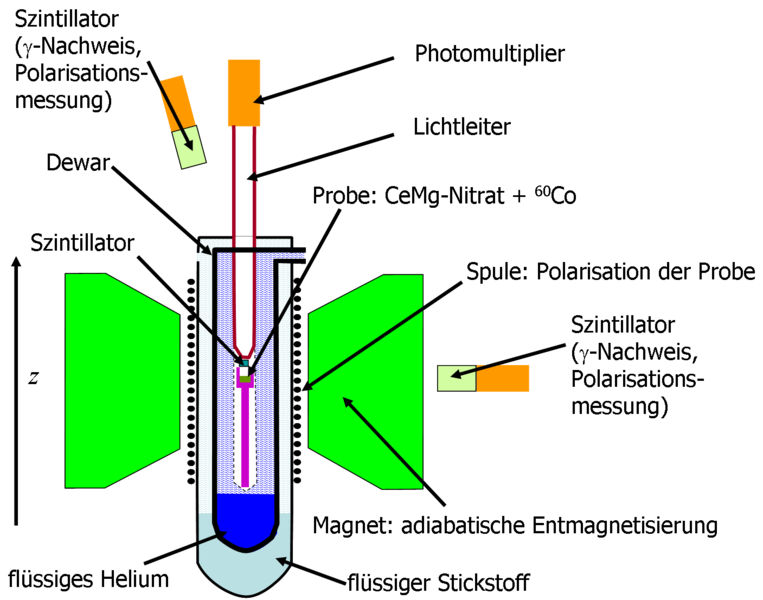
\includegraphics[height=7.0cm]{ressources/wu.png}
  \caption{Schematischer Aufbau des Wu-Experimentes \cite{wu}.}
  \label{fig:wu}
\end{figure}

Die Polarisation des Kernspins geschieht über die $\gamma$-Szintillatoren, da die Photonen vorzugsweise in Spin-Richtung emmitiert werden.
Der Nachweis der Elektronen geschieht direkt über den Szintillatorkristall über Photomultiplier.
Um die Parität untersuchen zu können wird das gesamte Experiment mit zwei verschiedenen Ausrichtungen des Magnetfeldes und somit mit zwei verschiedenen Vorzugsrichtungen der Spins durchgeführt.

\subsection{Experimentelle Ergebnisse und Konsequenzen}
Experimentell konnte nachgewiesen werden, dass die Kernspins hinreichend polarisiert werden konnten.
Zudem wurde gezeigt, dass die Elektronen vorzugsweise gegen die Richtung des Kernspins des Kobalts emmitiert werden.
Dies entspricht einer Verletzung der Parität und bestätigte somit die These von Tsung-Dao Lee und Chen Ning Yang.
Spätere Experimente wiesen quantitativ nach, dass die Parität tatsächlich maximal verletzt ist.
Zudem folgte die theoretische Erkenntnis, dass die schwache Wechselwirkung eine V-A-Struktur besitzt:
Sie koppelt nur an linkshändige Teilchen und rechtshändige Antiteilchen, was die maximale Paritätsverletzung erklärt.

\subsection{Diskussion zum Vortrag}
Als Frage wurde gestellt, ob die Suche nach Paritätsverletzung in anderen Wechselwirkungen ebenfalls durchgeführt wurde.
Hierbei ergab sich die Antwort, dass bis heute nach paritätsverletzenden Anteilen außerhalb der schwachen Wechselwirkung gesucht wird.

Da Kobalt zwei unteschiedliche $\beta^-$-Zerfallsmoden in Nickel besitzt, kam die Frage auf wie diese Unterschiede experimentell berücksichtigt wurden.
Dies war möglich und wurde realisiert, da die Szinzillatoren auf die festen Energien der Photonen ausgerichtet werden können.

Zuletzt wurde über technische Details der Kühlung diskutiert.
Hierbei wurde das Pumpen erwähnt, welches genutzt wurde, um eine Kühlung auf bis zu $\SI{1}{\kelvin}$ zu ermöglichen.

\newpage


\section{Die Entdeckung des Gluons}

\chapterauthor{Dominik Hellmann, 09.11.2018}

\subsection{Theoretische Grundlagen der Quantenchromodynamik}
Die Quantenchromodynamik (QCD) ist die Quantenfeldtheorie der starken Wechselwirkung, d.h. der Kraft, die für das Zusammenhalten der Quarks in Hadronen verantwortlich ist.
Grundlage für die QCD ist die Yang-Mills-Theorie, welche eine im Jahre 1954 entwickelte Eichtheorie ist.
Dabei folgt die QCD aus der $SU(3)_\text{c}$-Symmetriegruppe, wobei hieraus die drei Farbladungen rot, grün, blau und die dazugehörigen Antifarben resultieren.
Die Farben sind dabei analog zu den elektrischen Ladungen der QED zu verstehen.

Analog zu den Photonen der QED existieren auch Eichbosonen der QCD, welche Gluonen heißen.
Aus der Gruppentheorie folgt, dass 8 Gluonen existieren, welche den Generatoren der $SU(3)_\text{c}$ entsprechen.
Gluonen sind masselose Vektorteilchen, welche jedoch im Kontrast zur QED ebenfalls Farbladung besitzen und dementsprechend an sich selbst koppeln können.
Hieraus folgt die asymptotische Freiheit als charakteristische Eigenschaft der QCD:
Durch Vakuumpolarisationen, dem sogenannten Anti-Screening, wird die Kopplungskonstante der QCD $\alpha_{s}$ klein für große Impulsübertäge. 
Hieraus folgt, dass die einzelnen Quarks bei großen Impulsübertägen, bzw. kleinen Abständen, als asymptotisch frei verstanden werden können.
Andereresits folgt als Charakteristikum das Confinement: Bei großen Abständen steigt das Potential der QCD linear an, d.h. die Kraft für das weitere Vergrößern des Abstandes wächst linear.
Wird der Abstand weiter vergrößert, so werden neue Teilchen in sogenannten Jets produziert, bis der Endzustand wieder farbneutral ist.
Dementsprechend können farbgeladene Teilchen nur in einem farbneutralen, gebundenen Zustand beobachtet werden.
Die entstehenden Jets können in einem Detektor als Ansammlung von Teilchen beobachtet werden, wobei die Messung der Impulse aller beobachteten Teilchen Rückschlüsse auf die Impulse der ursprünglichen Quarks zulässt.

\subsection{Historische Entwicklung}

Im Jahr 1964 wurden von Murray Gell-Mann erstmals Quarks als Bestandteile der Hadronen postuliert.
Hierbei stellen sich die Fragen, welche Kräfte diese Elementarteilchen zusammenhalten und welche Austauschteilchen diese Kraft vermitteln.
Weitere Hinweise auf eine mit der QCD verbundenen Quantenzahl stellten die $\Delta$-Baryonen sowie der $R$-Plot dar.
So ist die Wellenfunktion des $\Delta^{++}$-Baryons unter Vertauschung von zwei Quarks symmetrisch, falls nur die bisher bekannten Raum-, Flavor- und Spinanteile der Wellenfunktion berücksichtigt werden.
Dies steht jedoch im Widerspruch mit dem Pauliprinzip für Fermionen.
Die Einführung einer Farbe als Quantenzahl stellt den nötigen antisymmetrischen Anteil der Wellenfunktion bereit und löst somit dieses Problem.

Bei der Betrachtung des $R$-Plots wird die Häufigkeit der Produktion von Hadronen in $e^+ e^-$ Reaktionen in Abhängigkeit von der Schwerpunktsenergie betrachtet.
Hierbei ist das Verhältnis $R$ sensitiv auf das Vorhandensein von Farbladungen und sagt experimentell drei Farbladungen vorraus.

\subsection{Jetphysik am DESY}
Das DESY (Deutsche Elektron Synchrotron) ist ein Forschungszentrum für Teilchenphysik, welches 1959 in Hamburg gegründet wurde.
Der dort gebaute $e^+ e^-$ Collider PETRA (Positron-Electron-Tandeom-Ring Accelerator) wurde im Oktober 1978 in Betrieb genommen.
Mit einem Umfang von $U=\SI{2.3}{\kilo\metre}$ konnten im späteren Betrieb Schwerpunktsenergien von bis zu $\SI{47}{\giga\electronvolt}$ erreicht werden.
Eines der an diesem Collider arbeitenden Experimente war TASSO (Two Arm Spectrometer Solenoid).
Mithilfe des mit einem Magnetfeld durchsetzten Zentraldetektors war eine genaue Impulsmessung möglich, zur Geschwindigkeitsmessung wurde ein Flugzeitzählersystem verwendet.
In den beiden Armen des Detektors konnte durch drei Lagen von Schwellen-Cherenkovzählern, Schauerzählern sowie den Flugzeitzählerystemen eine sehr gute Teilchenidentifikation ermöglicht werden.

Die Jet-Rekonstruktion zu dieser Zeit konzentrierte sich insbesondere auf die Beobachtung von 2-Jet-Ereignissen, wie sie 1975 durch Feynman erstmals vorhergesagt und 1978 am DESY entdeckt wurden.
Im Rahmen des Cone-Algorithmus wird dabei eine Hauptjetachse gesucht und die Impulse entlang dieser Achse maximiert beziehungsweise die Impulse transversal zu der Hauptachse minimiert.
Um die Existenz von Gluonen in der QCD zu beweisen kann das Auftreten von 3-Jet-Strukturen verwendet werden.
Dies entspricht der Abstrahlung eines Gluons, wie in Abbildung \ref{fig:gluon} dargestellt ist.
\begin{figure}
  \centering
  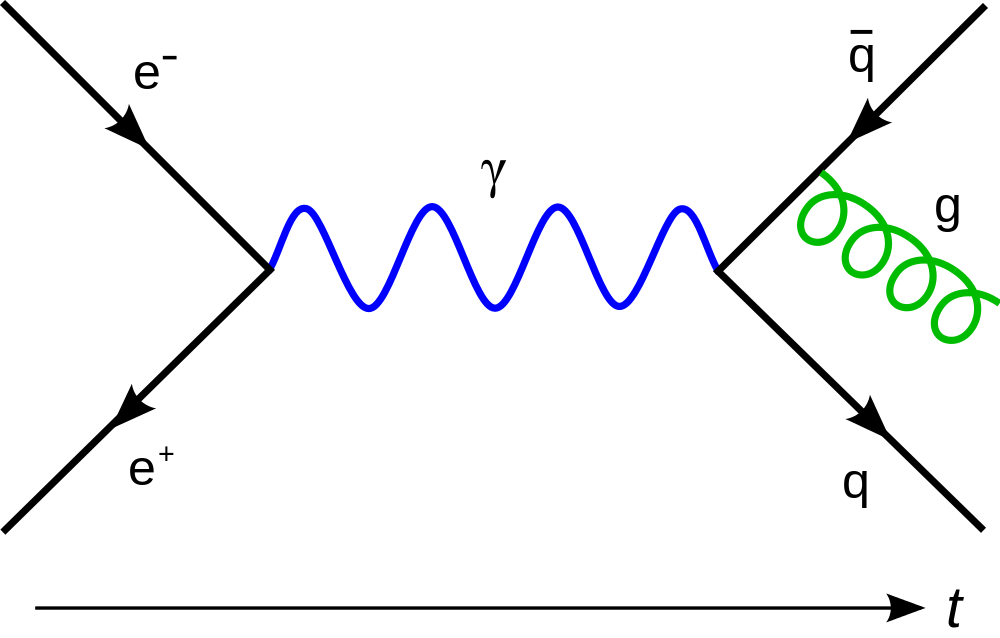
\includegraphics[height=4.0cm]{ressources/gluon.png}
  \caption{Abstrahlung eines Gluons in einer $e^+ e^-$-Kollision \cite{gluon}.}
  \label{fig:gluon}
\end{figure}
Bei einem ausreichend großen Tansversalimpuls des Gluons entsteht ein dritter Jet, der im Detektor nachgewiesen werden kann.

\subsection{Analyse der Jets der TASSO-Kollaboration}
Die Analyse der Jets wurde von der TASSO-Kollaboration bei verschiedenen Schwerpunktsenergien durchgeführt. 
Dabei teilt sich die Analyse jeweils in verschidene Schritte auf.
Zunächst wird die Hauptjetachse durch das Maxmimeren des Impulses in die Jetachsenrichtung bestimmt.
Die Verteilung der Impulse transversal zur Hauptsachse wird nun untersucht, wobei hier einer energieabhängige Verteilung der Transveralimpulse beobachtet wurde, die mit der Schwerpunktsenergie zugenommen hat. 
Dies widerspricht den bisherigen naiven Partonmodellen und ließe sich beispielsweise über die Abstrahlung von Gluonen erklären.

Im nächsten Schritt werden die Breiten der einzelnen Jets untersucht.
Bei zwei rekonstruierten Jets wäre zu erwarten, dass jeweils nur ein Jet aufgrund von Gluonabstrahlung verbreitert ist und somit eine Asymmetrie zu beobachten ist.
Die Ergebnisse zeigen, dass die Asymmetrie für größere Schwerpunktsenergien ansteigt und somit für verschiedene Energien unterschiedliche Parameter der Quark-Parton-Modelle verwendet werden müssen.
Auch dieses Verhalten ist mit der Abstrahlung von Gluonen als Erklärung kompatibel.

Der letzte Schritt besteht darin, die Struktur der 3-Jet-Ereignisse eindeutig von den kolinearen 2-Jet-Ereignissen zu trennen.
Dabei müssen die drei beobachteten Jets aufgrund der Impulserhaltung in einer Ebene liegen, jedoch eine Abweichung von der kolinearen Struktur innerhalb dieser Ebene aufweisen.
Dazu wird aus den beobachteten Impulsen der Hadron-Impulstensor ermittelt.
Aus den Eigenvektoren dieses Tensors lassen sich die Größen $\left<p_T^2\right>_\text{in}$ und $\left<p_T^2\right>_\text{out}$ ermitteln welche jeweils angeben, wie stark die gemessenen Impulse aus der Ereignisebene herausragen bzw. wie stark die Impulse von der Hauptjetachse in der Ereigbnisebene abweichen.
Beobachtet wird, dass $\left<p_T^2\right>_\text{out}$ lediglich einen geringen Anstieg mit der Schwerpunksenergie aufzeigt, während sich $\left<p_T^2\right>_\text{in}$ bei höheren Energien nicht mehr korrekt mit dem naiven Quark-Parton Modell beschreiben lässt.
Dies deutet auf ein drittes farbgeladenes Teilchen im Endzustand, welches bei höheren Energien einen Jet erzeugt, wobei die Häufigkeit dieser Ereignisse nicht mehr mit statistischen Fluktuationen kompatibel ist.

Der somit bestätigten Existenz des Gluons folgte die Bestimmung seines Spins, welches laut Theorie den Wert $1$ besitzen sollte.
Als hiermit korrelierte Größe wurde 1980 der sogenannte Ellis-Karliner Winkel von der TASSO-Kollaboration gemessen und mit Simulationen für verschiedene Spins des Gluons verglichen.
Hierbei wurde eine gute Übereinstimmung mit der Annahme eines Vektorteilchens, d.h. Spin 1 des Gluons, ermittelt.
Es folgten weitere Spinmessungen der SLD Kollboration, die dieses Ergebnis bestätigten.

\subsection{Heutige Jetphysik und QCD-Forschung}

In der heutigen Jetphysik können in einem Ereignis aufgrund der höheren Schwerpunktsenergien der Beschleuniger deutlich mehr als zwei Jets beobachtet werden.
Hierzu werden effiziente und schnelle Rekonstruktionsalgorithmen benötigt, welche die Eigenschaften der Infrarot-Stabilität sowie der kollinearen Stabilität erfüllen müsen.
Dafür werden, im Vergleich zu den vorher verwendeten Cone-Algortihmen, heutzutage häufig sequentielle Cluster Algorithmen (beispielsweise $k_t$, anti-$k_t$ und Camebridge/Aachsen) verwendet.

Aktuelle Forschungsfragen der QCD sind beispielsweise die Existenz von Glueballs oder der Beitrag der Gluonen und verschiedenen Quarks zum Protonspin.

\subsection{Diskussion}
Im Anschluss des Vortrages wurde gefragt, inwiefern sich die unterschiedlichen Spinmessungen des Gluons der verschiedenen Kollaborationen unterschieden haben.
Beim Folgeexperiment der SLD Kollaboration wurde durch höhere Schwerpunktsenergien und einen besseren Detektor eine höhere Auflösung und somit eine genauere Messung ermöglicht.

Zudem wurde gefragt, ob andere Kandidaten neben der QCD zur Erklärung der starken Wechselwirkung existierten.
Zwar wäre es möglich gewesen, einige Ergebnisse der Experimente zur Suche nach Gluonen durch einen weiteren Quarkflavor zu erklären - dies wurde jedoch bereits früh durch andere Experimente bei den geringen, hier genutzen Schwerpunktsenergien ausgeschlossen.
Eine generelle alternative theoretische Erklärung der starken Wechselwirkung exisiterte jedoch nicht.
\newpage


\section[Die J/Psi-Entdeckung]{Die $J/\Psi$-Entdeckung}

\chapterauthor{Jan Langer, 16.11.2018}

\subsection{Historische Einordnung und Quarkmodelle}

Die Entdeckung des $J/\Psi$ im Jahre 1974 gilt als Nachweis der Existenz eines 4. Quarks, dem Charm-Quark ($c$), sowie als allgemeine Bestätigung der Quark-Theorie.
Es handelt sich dabei um ein flavour-neutrales Meson, welches aus einem $c$ sowie einem $\overline{c}$ besteht.
Bereits im Jahr 1961 wurde der sogenannte Eightfold Way (Achtfache Weg) von Gell-Mann und Zweig vorgeschlagen, um die Teilchen mit der 1953 eingeführten Quantenzahl der Strangeness systematisch anzuordnen.
Hierbei werden die Mesonen, welche aus den zu diesem Zeitpunkt bekannten Quarks $u$, $d$ und $s$ bestehen, in einem Oktett sowie die Baryonen in einem Dekuplett angeordnet.
Dies entspricht einer Flavour $SU(3)$-Symmetrie, die annähernd zwischen den Quarks gültig ist.
Die Entdeckung des anhand diesem Modell postulierten $\Omega^-$-Quarks im Jahre 1964 festigte diese Theorie.


Im Jahr 1970 trat ein theoretisch unerwartetes Messergebnis im Zerfall von $K^0_\text{L}$-Mesonen auf, welches den sogenannten GIM-Mechanismus motivierte:
So konnte es bisher nicht erklärt werden, wieso der experimentell bestimmte Wert
\begin{align*}
	\frac{\Gamma\left( K^0_\text{L} \to \mu^+ \mu^- \right)}{\Gamma\left( K^0_\text{L}  \to \text{all}\right)} = \left(\num{9.1+-1.9}\right) \cdot \num{e-9}
\end{align*}
so gering ist.
Der von Glashow, Iliopoulus und Mainani beschriebe GIM-Mechanismus erklärt die Unterdrückung dieses Zerfalles durch eine destruktive Interferenz in Loop-Diagrammen erster Ordnung. Diese tritt durch die Einführung eines vierten Quarks, dem $c$-Quarks, auf.

Der Nachweis des $c$-Quarks über das $J/\Psi$ im Jahre 1974 bestätigt diese theoretische Erklärung, die bereits 1973 zur Erklärung der CP-Verletzung auf 3 Quarkfamilien erweitert wurde.

\subsection{Die Experimente am SLAC und BNL}
Das $J/\Psi$ wurde durch zwei unabhängige Experimente, dem Stanford Linear Accelerator Center (SLAC) und dem Brookhaven National Laboratory (BNL), entdeckt.
Die Entdeckung wurde auf einer gemeinsamen Pressekonferenz am 11. November 1974 offiziell bekannt gegeben.

Das Experiment am BNL, welches von Samuel Chao Chung Ting geleitet wurde, war ein fixed-target Experiment zur Suche nach Vektor-Mesonen und zur Untersuchung von deren Eigenschaften.
Der Beschleuniger konnte Protonen auf eine Energie von \SI{33}{\giga\electronvolt} beschleunigen, der Detektor war ein Zwei-Arm-Spektrometer.
Das Experiment am SLAC hingegen, unter Leitung von Burton Richter, war ein $e^+ e^-$-Speicherring mit dem Ziel, Hadronproduktion bei möglichst genauer Energie zu untersuchen.
Hierbei sollte insbesondere das Verhältnis $R$, d.h. der Anteil der Hadronproduktion bei Elektron-Positron Kollision, gemessen werden.
Der genutzte Detektor Mark1 war ein $4\pi$-Detektor, die maximale Schwerpunktsenergie im Schwerpunktsystem betrug $\SI{8}{\giga\electronvolt}$. 

\subsection{Ergebnisse der Experimente}

Der Peak in den Daten bei ca. $\SI{3.1}{\giga\electronvolt}$, welches der $J/\Psi$-Resonanz entspricht, wurde zunächst im August 1974 am BNL beobachtet, wobei zunächst auf eine Publikation verzichtet wurde.
Da es sich um einen $pp$-Collider handelt, war mussten bei den Analysen zur Trennung von Signal und Untergrund Spurrekonstruktionen durchgeführt werden.
Zudem wurden bei der Analyse der Daten viele Gegenproben durchgeführt, beispielsweise durch die Änderung der Magnetströme, der Strahlintensität oder der Targetdicke.

Anfang November entdeckte auch das SLAC eine Erhöhung des Wirkungsquerschnittes $\sigma\left(e^+ e^- \to \text{Hadronen}\right)$ im passenden Energiebereich, nachdem die Energie des Colliders auf die Resonanzenergie zurückgefahren wurde.
Feinere Messschritte ergaben eine deutliche Erhöhung des Wirkungsquerschnittes für hadronische Endzustände und somit den Nachweis der $J/\Psi$-Resonanz.

Während das SLAC-Experiment eine obere Grenze der Zerfallsbreite von $\Gamma \leq \SI{1.3}{\mega\electronvolt}$ angeben konnte, waren die Ergebnisse von BNL mit $\Gamma = 0$ kompatibel.
Die mit der schmalen Zerfallsbreite verbundene hohe Lebensdauer konnte mit den bisherigen Quarks nicht erklärt werden.
Die Deutung Tings, dass das $J/\Psi$ dementsprechend aus der Kombination $c\overline{c}$ besteht, bestätigte sich bereits nach einem Jahr.

Im Jahre 1976 erhielten beide Experimentatoren den Nobelpreis für die Entdeckung des $c$-Quarks.
Bereits wenige Tage nach der $J/\Psi$-Entdeckung folgte die Entdeckung vieler weiterer Resonanzen - diese Zeit wird historisch auch als Novemberrevolution bezeichnet.

\subsection{Diskussion}
In der Diskussion wurde gefragt, wie genau es zu der Novemberrevolution nach der $J/\Psi$-Entdeckung gekommen ist.
Nach der Publikation wurde genauer in den entsprechenden Energiebereichen gesucht, zusätzlich sind die Experimente im Laufe der Zeit besser geworden.

Zudem wurde der qualitative Unterschied zwischen einer $e^+ e^-$-Maschine und einem $pp$-Experiment besprochen.
Bei einem $e^+ e^-$ Collider handelt es sich um ein Präzisions-Experiment: Die Reaktionen sind sehr sauber und können durch einfaches Zählen der Endprodukte gut verstanden werden.
Dafür ist bei diesen Experimenten nur eine feste Schwerpunktsenergie vorhanden, die für neue Entdeckungen fortlaufend verändert werden muss.
Bei $pp$-Experimenten müssen die Endzustände aufgrund der hadronischen Reaktionen aufwendig rekonstruiert werden.
Dafür kann, aufgrund der an den Reaktion beteiligten Partonen, gleichzeitig ein großes Energiespektrum untersucht werden.
\newpage


\section{Entdeckung von Neutrinos}

\chapterauthor{Felix Geyer, 23.11.2018}

\subsection{Historische Postulierung des Neutrinos}
Historisch betrachtet geht die erste Postulierung des Neutrinos auf die Betrachtung des $\beta^-$-Zerfalles um das Jahr 1930 zurück.
Zu dieser Zeit wurde der $\beta^-$-Prozess als Zweikörperzerfall $\ce{n -> p + e^-}$ betrachtet, was kinematisch zu einer diskreten Energie des Elektrons führt.
Entgegen dieser Vorhersage wurde jedoch ein kontinuierliches Energiespektrum für das Elektron gemessen.
Zusätzlich wird die Drehimpulserhaltung bei dieser Betrachtung des Zerfalles verletzt.

Dies führte zu der ersten Vorhersage eines Neutrinos durch Pauli, der ein sehr leichtes Teilchen mit halbzahligen Spin vorhersagte, welches beim $\beta^-$-Zerfall zusätzlich zum Proton und Elektron entsteht.
Bei einem Dreikörperzerfall wäre das gemessene kontinuierliche Energiespektrum des Elektrons erklärbar.
Paulis Theorie zum $\beta^-$-Zerfall wurde 1934 erstmals publiziert.

\subsection{Experimenteller Nachweis des Neutrinos}
Im Laufe der Zeit existierten mehrere verschiedene Ideen und Experimente, um einen Nachweis von Neutrinos zu ermöglichen.
Führend bei der Entwicklung dieser Ideen und Experimente waren Frederick Reines und Clyde Cowan.

Die grundlegende Idee bestand darin, Neutrinos durch den Neutroneneinfang $\overline{\nu_e} + p \rightarrow n + e^+$ nachzuweisen.
Um eine große Neutrinoquelle zu erhalten und somit den vorhandenen, großen Untergrund zu eliminieren sollte eine Atombombe gezündet werden.
Hierbei spielte auch die Tatsache eine Rolle, dass der theoretisch berechnete Wirkungsquerschnitt dieser Nachweisreaktion bereits kurz nach der Veröffentlichung von Fermis Theorie zum $\beta$-Zerfall zu $\approx \SI{1e-20}{\barn}$ berechnet wurde, d.h. die Reaktion war äußerst selten.
Als Detektor sollte ein flüssiger Szintillationsdetektor verwendet werden, welcher auch auf größeren Skalen genutzt werden kann.
Durch Paarvernichtung des Positrons aus dem $\beta^-$-Zerfall mit vorhandenen Elektronen entstehen zwei Photonen, die im Szintillationsdetektor Lichtblitze verursachen.
Diese können nun durch Photomultiplier detektiert werden.

Um auf den Aufwand der Zündung einer Atombombe verzichten zu können, und somit auch eine einfachere Reproduzierbarkeit des Experimentes zu ermöglichen, entstand eine verbesserte Idee für den experimentellen Aufbau:
Hierbei sollte auch das beim $\beta^-$-Zerfall entstehende Neutron nachgewiesen werden indem die beim Kerneinfang entstehende $\gamma$-Strahlung im Detektor nachgewiesen wird.
Dafür wurde mit Cadmium versetztes Wasser als Reaktionsmedium verwendet.
Der verzögerte Nachweis von Positron und Neutron, d.h. die Koinzidenz, wäre eine eindeutige Signatur für Neutrinos und ermöglicht eine starke Reduzierung von Untergrundereignissen.
Diese Verringerung des Untergrundes erlaubte es einen Kernreaktor als Neutrinoquelle zu verwenden.
Der Detektor wurde dabei knapp $\SI{2}{\metre}$ vom Reaktor entfernt aufgestellt.
Um die direkt vom Reaktor erzeugten Neutronen abzuschirmen wurde der Detektor in eine Borax-Wasser-Lösung getaucht.
Zudem wurde eine Anti-Koinzidenz für den Ausschluss kosmischer Strahlung sowie Quecksilber und Blei gegen zur Abschirmung gegen natürliche Radioaktivität verwendet.
Die Messungen wurden insbesondere durch einen nach wie vor zu hohen Untergrund durch kosmische Strahlung sowie elektronisches Rauschen, vor allem durch die vielen Photomultiplier, erschwert.
Das Experiment wurde sowohl bei eingeschaltetem als auch bei ausgeschaltetem Reaktor durchgeführt, wobei auch in letzterem Fall eine Signalrate nachgewiesen wurde.
Dieser Hintergrund konnte später als kosmische Strahlung identifiziert werden.

Um eine aussagekräftige Messung zu erhalten wurde das Experiment im November 1955 an einem Reaktor im Savannah River Plant neu aufgebaut.
Einerseits besaß dieser Reaktor eine hohe Reaktorleistung und somit einen hohen Antineutrinofluss, zudem befand sich der Detektor $\SI{12}{\metre}$ unter der Erde, was eine bessere Abschirmung von komischer Strahlung ermöglichte.
Als Reaktionsmedium wurde ein mit Cadmium versetzter Wassertank verwendet, welcher oben und unten von zwei Szintillatoren umgeben war.
Die Messungen wurden über 100 Tage durchgeführt, die ermittelte Signalrate betrug $\SI{3.0+-0.2}{\per\hour}$.
Um nachzuweisen, dass der erste Impuls tatsächlich durch die Positronen auftritt, wurde testweise eine Bleischicht zwischen dem Wassertank und einer der Szintillatoren aufgestellt, was zu einer geringeren Detektion von ersten Impulsen in diesem Szintillator führt.
Zur Kontrolle des durch Neutronen auftretenden zweiten Impulses wurde das Cadmium aus dem Wassertank entfernt, wodurch die Rate komplett verschwindet da kein Neutroneneinfang mehr stattfindet.
Die Resultate dieses Experimentes gelten somit als Entdeckung des Neutrinos.
Reines erhielt 1995 den Nobelpreis für seine Arbeiten im Bereich der Neutrinophysik.

\subsection{Weitere Entdeckungen und Experimente der Neutrinophysik}
Während beim Savannah River Experiment Elektronneutrinos untersucht wurden, konnte 1962 von Leon Lederman, Melvin Schwatz und Jack Steinberger am Alternating Gradient Synchrotron auch das Myonneutrino nachgewiesen werden.
Hierfür wurden Pionen mithilfe eines Fixed Target Experimentes erzeugt.
Diese zerfielen in Myonen sowie Myonneutrinos, wobei dieser Neutrinobeam von einer Stahlwand abgeschirmt wurde.
Im Gegensatz zu den Myonen können die Neutrinos diese Wand passieren und durch Kerneinfang als entstehende Myonen nachgewiesen werden.

Im Jahre 2000 wurde durch das DONUT-Experiment am Fermilab ebenfalls das Tauneutrino nachgewiesen.
Erschwerend bei dessen Nachweis ist die geringe Lebensdauer der entstehenden Tauonen beim Einfang von Neutrinos durch Neutronen.

Heutige betriebene Neutrinoexperimente sind beispielsweise ANTARES, IceCube oder (Super-)Kamiokande.
Diese Experimente dienen verschiedenen Zwecken wie dem Nachweis von atmosphärischen, solaren oder kosmischen Neutrinos der unterschiedlichen Neutrinofamilien.
\newpage


\section{Neutrinooszillationen}

\chapterauthor{Hubertus Kaiser, 30.11.2018}

\subsection{Das solare und das atmosphärische Neutrinoproblem}

In den 1960er Jahren trat mit dem solaren Neutrinoproblem erstmals eine Beobachtung auf, welche nicht ohne Probleme mit den bisher im Standardmodell als masselos angenommenen Neutrinos gelöst werden konnte.
Heutzutage ist bekannt, dass Neutrinos nicht nur in drei Generationen ($\nu_e, \nu_\mu, \nu_\tau$) auftreten, sondern aufgrund ihrer geringen Masse auch zwischen diesen Generationen oszillieren können.
Bereits früh war bekannt, dass die Sonne bei seiner Energiegewinnung Elektronneutrinos produziert.
Mit dem Homestake Experiment, welches 1970 mit seiner Messung begann, wurde die Anzahl an Neutrinos aus der Sonne gemessen.
Hierzu befand sich $\SI{1.5}{\kilo\metre}$ unter der Erde ein Tank aus $\SI{380}{\cubic\meter}$ $\ce{C2Cl4}$, in welchem aus der Umwandlungsreaktion $\nu_e + ^{37}\ce{Cl} \rightarrow ^{37}\ce{Ar} + e^-$ durch genaues Zählen der entstandenen Argon-Atome die solaren Neutrinos gemessen werden konnten.
Das Ergebnis stand im Widerspruch mit dem solaren Standardmodell, welches bis zu diesem Zeitpunkt jedoch gute Aussagen über die Eigenschaften der Sonne wie Energiespektrum, Helligkeit oder Temperatur machte.
Betrachtet man das Ergebnis über die komplette Messphase (1970 bis 1994), so ist die Anzahl der gemessenen Neutrinos um einen Faktor $3$ zu gering.
Auch weitere spätere Experimente wie Kamiokande oder Gallex, jeweils mit anderen Energieschwellen für die Neutrinos, konnten diese Abweichungen bestätigten.

Beim atmosphärischen Neutrinoproblem werden die Neutrinos betrachtet, welche bei Reaktionen von astrophysikalischen Teilchen mit der Atmosphäre entstehen.
Hierbei wurde das beobachtete Verhältnis von $\nu_\mu$ zu $\nu_e$ im Vergleich zu theoretischen Erwartungen von vielen Experimenten als wesentlich geringer gemessen.

Beide Probleme können letztendlich durch die Einführung von Neutrinooszillationen gelöst werden:
Hierbei können Neutrinos einer bestimmten Familie während der Propagation ihre Familie wechseln, wodurch sich die beobachteten Verhältnisse verändern.
Die erste Theorie von Neutrinooszillationen geht auf Bruno Pontecorvo im Jahre 1957 zurück.

\subsection{Beobachtung von Neutrinooszillationen}
Zur Beobachtung der Neutrinooszillationen wurden weitere Experimente durchgeführt.
So wurden mit dem Sudbury Neutrino Observatory, einem Detektor bestehend aus einem großen $\ce{D2O}$-Tank sowie Photomultipliern, von 1999 bis 2006 Daten aufgenommen.
Elektronneutrinos können bei diesem Experiment über geladene Ströme das Neutron im Deuterium zu einem Proton umwandeln, wobei sich das Neutrino in ein Elektron umwandelt.
Dieses Elektron kann wiederum über sein Cherenkovlicht im Wasser nachgewiesen werden.
Während diese Reaktion nur durch Elektronneutrinos ausgelöst werden kann, können Neutrinos aller Familien über neutrale Ströme ($d + \nu \rightarrow n + p + \nu$, Disintegration) sowie elastische Elektronstreuung ($\nu + e^- \rightarrow \nu + e^-$) wechselwirken und somit nachgewiesen werden.
Somit konnten die fehlenden Elektronneutrinos aus dem solaren Neutrinoproblem als Neutrinos anderer Generationen gemessen werden.
Auch die Ergebnisse von Super-Kamiokande, einem Experiment mit ähnlichem Aufbau, sind mit der Theorie von Neutrinooszillationen gut kompatibel.

Für diese Beobachtungen erhielten Takaaki Kajita (Super-Kamiokande) und Arthur McDonald (Sudbury Neutrino Observatory) 2015 den Nobelpreis für die Entdeckung von Neutrinooszillationen.

\subsection{Theorie der Neutrinooszillationen und weitere Messungen}
Ähnlich wie bei der CKM-Matrix für die Quarkgenerationen existiert die PMNS-Matrix, welche die Masseneigenzustände an die Eigenzustände der schwachen Wechselwirkung koppelt.
Sie besitzt 3 freie Parameter sowie eine Phase, dessen Bestimmung bzw. Messung wichtig für das genaue Verständnis der Neutrinooszilationen ist.
Relevant dabei ist insbesondere, dass die Oszillationswahrscheinlichkeit nicht nur von der zurückgelegten Strecke, sondern auch von den Massendifferenzen der Neutrinos abhängig ist:
Ohne Neutrinomassen können keine Neutrinooszillationen existieren, so dass der Nachweis von Oszillationen direkt aussagt, dass Neutrinos eine von null verschiedene Masse besitzen.
Dies entspricht bereits einer Erweiterung des Standardmodells der Teilchenphysik.

Experimente wie das T2K-Experiment sollen die Parameter der PMNS-Matrix bestimmen.
Bei diesem Experiment wird ein durch einen Strahl beschleunigter Protonen erzeugter Neutrinobeam verwendet, und mittels eines nahen sowie eines fernen Detektors (Super-Kamiokande) werden die während der propagierten Strecke auftretenden Oszillationen untersucht.

Ein weiterer Effekt in Kombination mit Neutrinooszillationen ist der Mikheyev-Smirnov-Wolfenstein-Effekt: 
Er besagt, dass sich das Oszillationsverhalten in Materie von dem im Vakuum unterscheidet.
Diese Asymmetrie konnte durch Experimente wie Kamland und Super-Kamiokande mittels einer tageszeitabhängigen Messung bestimmt werden:
Je nachdem, wie viel Erdmaterial zwischen der Sonne und dem Detektor liegt (was tageszeitabhängig ist), verhalten sich die Oszillationen unterschiedlich.

Relevant ist dieser Effekt ebenfalls für das Problem der sogenannten Massenhierarchie der Neutrinos:
Die Beträge der Massendifferenzen der Neutrinos können über Messobservablen bestimmt werden.
Das Vorzeichen kann jedoch über den MSW-Effekt lediglich für einen Abstand bestimmt werden, d.h. für $\Delta m_{21}$. Ob sich die Masse des dritten Neutrinos relativ oberhalb oder unterhalb dieser beiden Massen befindet, ist, genauso wie die absoluten Massen, unbekannt.

In der Neutrinophysik ist somit insbesondere die Messung der Matrixelemente Thema der aktuellen Forschung.
Zudem sollen die Massendifferenzen genauer bestimmt werden.
Auch neue Eigenschaften, wie die Existenz von sterilen Neutrinos oder Neutrinos als Majoranateilchen, werden bis heute untersucht.

\subsection{Diskussion}

In der Diskussion zum Vortrag wurden insbesondere Ergebnisse sowie experimentelle Besonderheiten besprochen.
Zudem kam die Frage auf, wieso in der Atmosphäre mehr $\mu^+$ als $\mu^-$ Teilchen auftreten.
Diese Frage lässt sich dadurch beantworten, dass insbesondere Protonen als kosmische Strahlung auf die Atmosphäre treffen und somit aufgrund der Ladungserhaltung insgesamt mehr positiv als negativ geladene Teilchen auftreten.
Anschließend an diese Frage wurde besprochen, wieso das Verhältnis von $\mu^+$ zu $\mu^-$ zu höheren Energien ansteigt.
Dies liegt daran, dass die Teilchen höherer Energien insbesondere als Primärteilchen aus der Reaktion mit der Atmosphäre auftreten, und somit vornehmlich positiv geladen sind.
\newpage

\bibliographystyle{abbrv}
\bibliography{summary}

\end{document}

